\chapter*{\FontH{\Huge Der kleine Pirat Winnimon}}
\addcontentsline{toc}{chapter}{Der kleine Pirat Winnimon}
\section*{\center $\skull$ Die Prüfung $\skull$}
\lettrine[lines=3]{\color{red}W}{ie} jeder andere Pirat auch, war Winniemon nicht schon immer ein Pirat. Genau wie du und ich war er zunächst ein kleiner Junge, der höchstens einmal mit dem Boot seines Opas zum Angeln auf dem Meer gewesen ist. 

\todo{Aye. Dorf der Waisen. Piratengesetze-Mitspracherecht, Spanier, Klabautermann, Jolly Roger, Krähennest, Kombüse, Smutje, Papagei, Seemannsknoten, Bukanier}
Aber auch das war er nicht besonders oft, denn Winnimon hatte ein Problem, für das er sich sehr geschämt hat. Er konnte nicht schwimmen! Piraten müssen aber schwimmen können, das ist klar. Piraten müssen nämlich ständig Mutproben machen, da kann es schon einmal vorkommen, dass man mit verbundenen Augen und einem Messer im Mund auf der Reeling balancieren muss. Und wenn man dann den kleinsten Fehler macht, liegt man im Meer.

Wenn man nicht schwimmen kann, sollte man sich lieber einen anderen Beruf aussuchen. Das kam für Winnimon aber nicht in Frage. Undenkbar! Der Vater war ein Pirat und sein grosser Bruder war auch einer. Und was viel wichtiger war: alle seine Freunde wollten Pirat werden. Und die konnten schwimmen, die brauchten sich keine Sorgen zu machen.

Wenn man auf einem Piratenschiff anheuern möchte, muss man drei Prüfungen bestehen. Erstens muss man fluchen können wie ein alter Papagei. Das klappte bei Winnimon ausgezeichnet, jedenfalls fand das seine Mutter, die aber allgemein nicht viel für Flüche übrig hatte. 

\enquote{Du dreifach stinkender Pups einer blinden Robbe} war Winnimons Lieblingsfluch. Den hatte er erst einmal gesagt, als grosser Bruder ihm einmal zum Frühstück eine leere Eischale hingesetzt hatte. Die Mutter hätte ihm fast eine Ohrfeige gegeben, was aber ein gutes Zeichen war. Denn seitdem wusste er, welchen Fluch er zur ersten Piratenprüfung fluchen würde. Den hatte er lieber nicht noch einmal geflucht, nicht dass ihm den noch jemand von seinen Freunden klaut!

Die zweite Prüfung war auch nicht so schwer. Man musste lesen und schreiben können. Erstens musste man der Mutter eine Flaschenpost schicken können, falls zum Beispiel die Socken so alt waren, dass sie neue schicken musste oder wenn man einfach Heimweh hatte. Das darf man sogar als Pirat haben, der gerade durch ferne Meere kreuzt. Und man musste natürlich Schatzkarten lesen können. Wenn da steht \enquote{Der Schatz liegt auf der Insel Woladimadudistan} ist das schon besser, sonst muss man den Schatz auf allen Inseln suchen und von denen gibt es viele. Aber Winnimon war zwar nicht so schlau wie die lange Druda aus seiner Klasse, aber Lesen und Schreiben klappten prima. Kein Problem also, die zweite Piratenprüfung.

Es blieb nur die Sache mit dem Schwimmen. Nicht dass Winnimon es nicht immer wieder einmal probieren würde. Aber er zappelte nur, der grosse Bruder lachte, der Vater war ärgerlich und nach dem zweiten Schluck Wasser, dass er unfreiwillig getrunken hatte, gab er immer auf. Wie machten das die anderen bloss? Wen er probierte, nicht mehr mit den Beinen auf dem Boden zu stehen, ging der Kopf automatisch unter Wasser. Schrecklich! Er hatte gar keine Zeit, überhaupt nur einmal einen Schwimmzug zu probieren.

In dem kleinen Dorf, in dem er wohnte, herrschte grosse Aufregung. Ein Piratenschiff hatte sich angekündigt, in drei Wochen schon sollte es da sein. Es wurden Jungen gesucht, die mit auf See wollten. Und Winnimon wollte. Und wie er wollte! Pirat sein, das ist das Grösste! Sofort machte er sich auf zum Meer, schwimmen üben. Noch drei Wochen, bis dahin musste das klappen, unbedingt. 

Am Strand waren schon die anderen Jungen versammelt, auch die, die nicht Pirat werden wollten. Sie hatten aus Brettern ein Floss gebastelt und spielten natürlich Pirat. Sie sprangen von Floss ins Wasser und schwammen um die Wette. Winnimon zog seine Badehose und watete vorsichtig ein paar Schritte ins Meer. Die Wellen schwapptem ihm gegen den Bauch. Er wusste nicht einmal, wie er anfangen sollte zu üben. Er wartete auf ein Tal zwischen zwei Wellen und kniete sich hin. Aber schon spülte die nächste Welle ihn im hohen Bogen ans Ufer zurück. 

Den anderen war das traurige Schauspiel natürlich nicht entgangen. Lachend und schreiend kamen sie angerannt und hänselten Winnimon.

\enquote{Seht Euch mal den an, der Schwimmt ein Sack voller Steine!} war noch das Harmloseste. Obwohl Piraten nie weinen, kullerten Winnimon ein paar Tränen über die Wangen. Nicht weil die anderen ihn gehänselt haben, das war nicht so schlimm, so was kommt vor, er hat ja auch schon mitgemacht. Das Schlimme war, dass sie ja Recht hatten. Er schwamm tatsächlich genau so wie ein Sack voller Steine: immer direkt nach unten.

Eine Hand legte sich auf seine Schulter. Die lange Druda stand hinter ihm. An jedem anderen Tag wäre Winnimon vor Scham im Erdboden versunken, wenn ein Mädchen ihn weinen sieht, aber heute war ihm alles egal. Schluchzend erklärte er ihr, warum er so weinen musste. Druda überlegte. 

\enquote{Also pass auf} sagte sie. \enquote{Ich bringe dir das Schwimmen bei. Aber Du musst dann auch etwas für mich tun. Versprichst Du das?}

Winnimon zögerte keinen Augenblick. \enquote{Alles, was Du willst!}

\enquote{Na gut, dann komm morgen früh zum Waldrand. Und bring zwei Rumfässer und ein Seil mit.}

Ausgerüstet mit den verlangten Dingen und einer frisch gewaschenen Badehose stand Winnimon schon am Waldrand, bevor es hell wurde. Druda kam pünktlich zum Sonnenaufgang und hatte nicht vergessen, etwas zum Essen mitzubringen. Als erstes sträkten sich die beiden, dann gingen sie zu dem kleinen Waldsee, der ein bisschen versteckt war.

\todo{Zeitformen anpassen}
\enquote{Hier wirst du schwimmen lernen} sagt sie. \enquote{Das Wasser hier ist ruhig, da kann man besser üben. So, und jetzt binden wir den Strick zwischen die beiden Fässer, aber so, dass noch etwas Platz dazwischen ist.}

Knoten konnte Winnimon schon sehr gut und so dauerte es nicht lange, bis er fertig war. Die Fässer sollten als Schwimmer dienen, er selbst legte sich auf die Seile dazwischen. So konnte er nicht untergehen. Druda zeigt ihm mit viel Geduld wie man schwimmt. Die Beine wie ein Frosch und die Arme wie ein Pfeil nach vorne und wie ein Bogen nach hinten.

Noch am selben Tag klappte das schon ganz gut und einen Tag später liessen sie die Fässer weg. Winnimon schwamm jeden Tag Und jedes Mal ein bisschen besser. Nach der ersten Woche waren beide zufrieden. Winnimon konnte schwimmen wie ein Fisch und ebenso gut tauchen.

Druda meinte: \enquote{Das Letzte, was Du noch lernen musst, ist einen ordentlichen Kopfsprung zu machen. Aber bevor ich dir den zeige, erinnere ich dich daran, was du mir versprochen hast. Jetzt musst du mir helfen.}

\begin{figure}[hb]
\centering
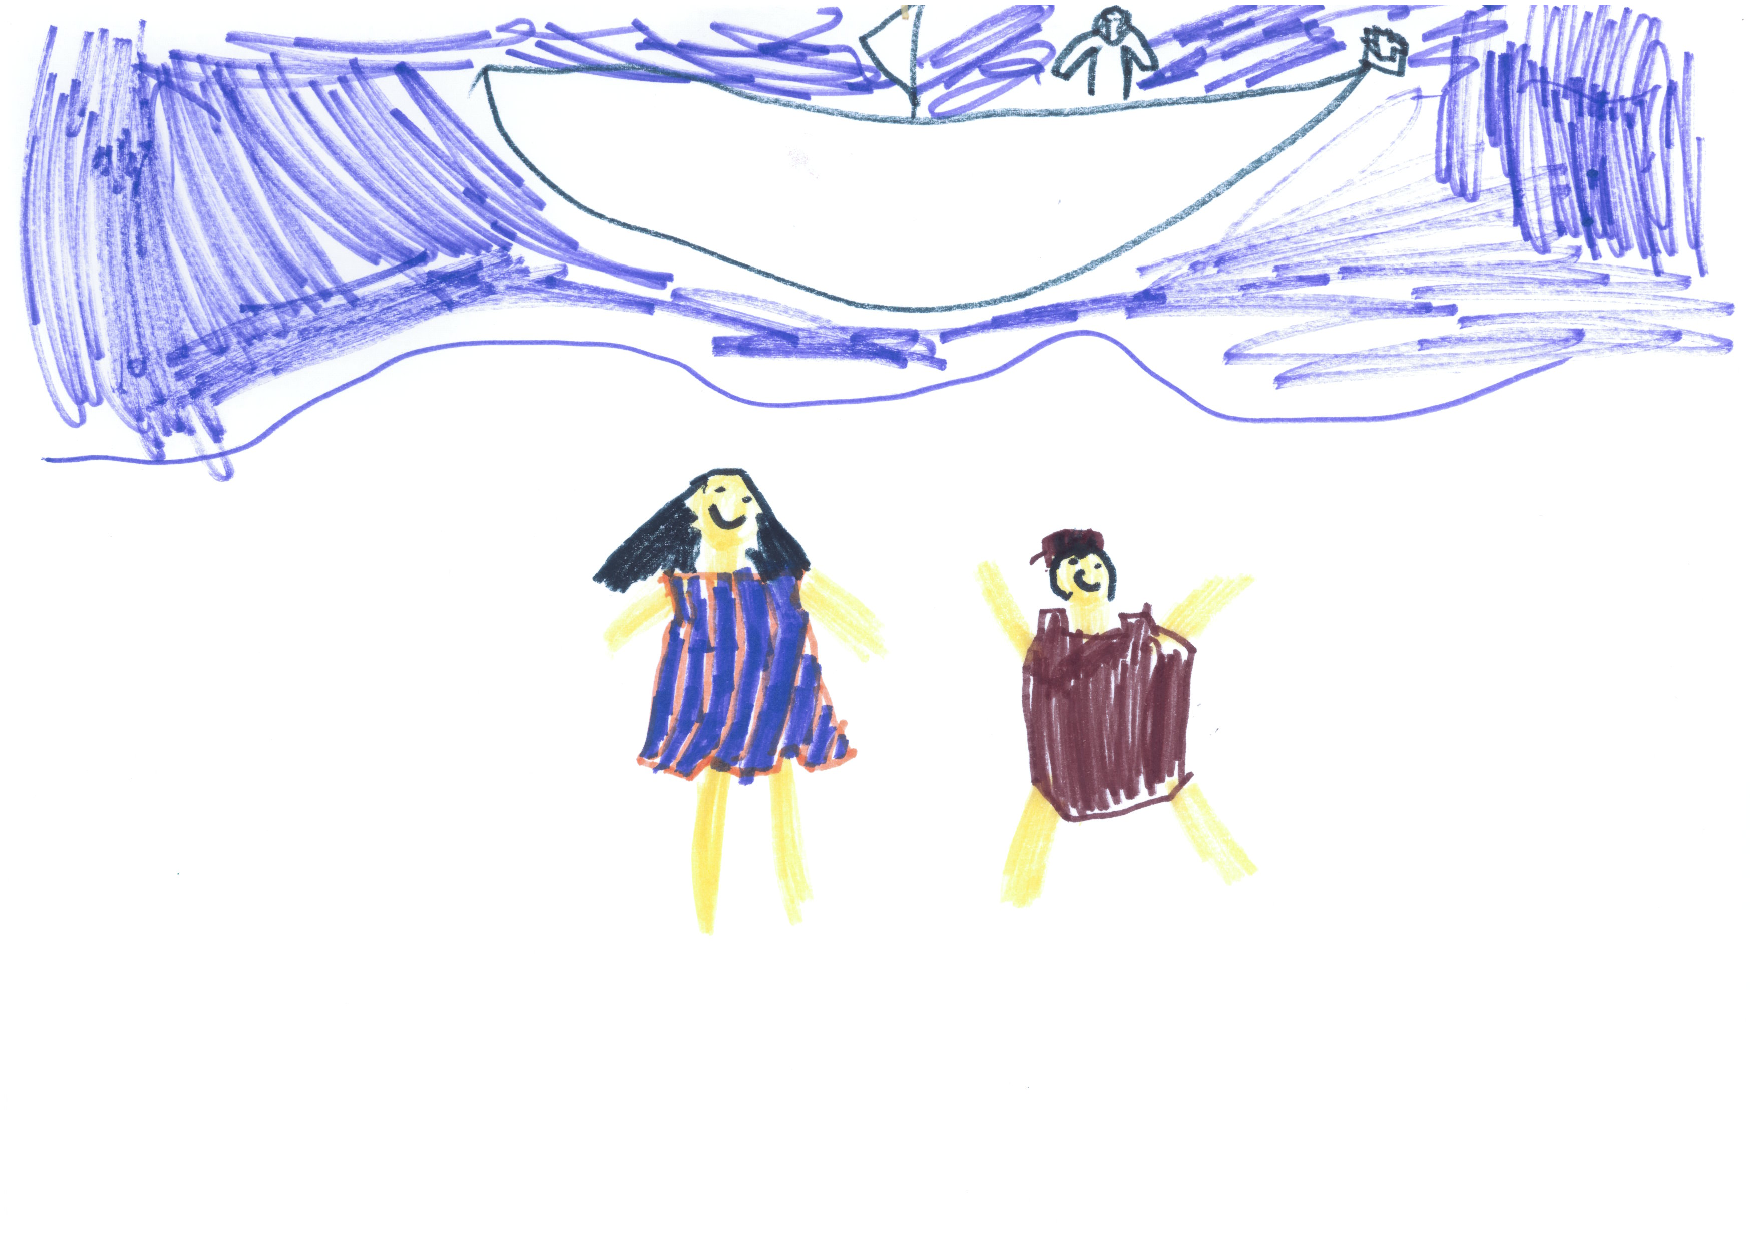
\includegraphics[width=.7\textwidth]{bilder/pirat1.pdf}
\end{figure}

Winnimon blickte fragend. Sie holte tief Luft und sagte: \enquote{Ich kann nicht fluchen. Mir fällt einfach kein Fluch ein. Du musst mir den besten Fluch verraten, den du kennst!}

\enquote{Aber warum willst du denn fluchen können?} Winnimon blickte fragend. \enquote{Du willst doch nicht etwa\dots?}

\enquote{Aber natürlich will ich auch Piratin werden! Meinst du ich will mein ganzes Leben hier verbringen? Ich will auch raus und die Welt sehen. Und jetzt hab ich dir geholfen, jetzt musst du mir helfen!}

Winnimon sah das sofort ein. Ihm ging es ja genauso. Und er zögerte nicht lange und verriet Drude seinen Lieblingsfluch. Das war er ihr schuldig, da gab es keine Frage. Ihm würde schon etwas einfallen.

Als beide zurück im Dorf waren, merkten sie gleich, dass etwas nicht stimmt. Vorbei am Haus von Winnimon sahen sie es auch schon. Ihm Hafen waren riesige Segel zu sehen und ganz oben auf dem höchsten Masten wehte die schwarze Fahne mit dem Totenkopf. Die Piraten waren da!

Sofort liefen die beiden hinunter zum Hafen. Das ganze Dorf hatte sich schon versammelt. Ein dicker Pirat stand in der Mitte der Menschenmenge auf einem Fass und rief:

\enquote{Liebe Leute. Mein Name ist Francisco San. Ich diene unter Barnabas Rotwild als erster Leutnant auf der Drachenblume, dem grössten Piratenschiff weit und breit. Wir sind gekommen, um zu fragen, ob jemand hier an Bord anheuern will. Wir nehmen zwei Schiffsjungen auf. Kommt mit uns, lernt die Welt kennen und werdet reich oder geht mit uns unter. Ihr alle kennt die drei Prüfungen. Aus all denen, die sie bestehen, nehmen wir zwei von euch auf. Freiwillige, tretet vor! Lang leben die Piraten!}

Alle Jungen und Mädchen waren sofort sehr aufgeregt, alle wollten mit. Nachdem sich die ersten getraut hatten vorzutreten, gaben sich auch Winnimon und Drude einen Ruck und stellten sich neben die anderen, alle in eine Reihe. Das alles so schnell gehen würde, hätten sie ja nie gedacht.

\enquote{Na dann wollen wir mal sehen.} Leutnant Francisco San schritt langsam die Reihe der Jugendlichen ab und zwirbelte dabei seinen Bart. \enquote{Ihr nehmt euch jetzt alle einen Stift und ein Stück Papier von dort drüben und schreibt folgende Wörter auf: Schatztruhe, Gewitter, arbeiten und Papagei.}

Die Prüfung war nur für zwei Jungen und ein Mädchen ein Problem, die ohne zu diskutieren den Stift hinlegten und aus der Reihe der Jugendlichen zurücktraten. Die waren schon durchgefallen. 

Bei der nächsten Prüfung, dem Fluchen, ging es sehr schnell zu. Jeder musste sich auf das Fass stellen und einmal so laut fluchen wie er konnte. 

\enquote{Dreibeiniger Hund}, \enquote{Vierauge}, \enquote{Vogelscheuche}, das waren so die Flüche die man hören konnte. Aber der Leutnant war nicht zufrieden. Die Flüche hätten alle schon einen längeren Bart als Kapitän Rotwild. Und wenn man so lange auf See ist und man immer die selben Flüche hört, wird einem echten Piraten sofort langweilig. Dann kamen Drude und Winnimon an die Reihe. Drude bestand den Test sofort mit mit dem {\it dreifach stinkenden Pups einer toten Ratte}. Sie war Winnimon sehr dankbar, denn mehr als Schwachkopf, aber da musste sie selbst zugeben, dass das sehr langweilig ist.

Winnimon brachte erst kein Wort heraus. So lange hatte er sich darauf verlassen, einen prima Fluch zu haben, dass er sich keinen neuen überlegt hatt. Wie angewurzrlt stand er auf dem Fass, aber dann brach es aus ihm heraus:

\enquote{Eitrige Warze am Bauch einer toten Ratte}. Der Leutnant lachte und sagte bestanden.

Danach waren nur noch drei Jugendliche im Rennen. Drude, Winnimon und ein weiterer Junge. Einer von denen die immer über Winnimon gelacht hatte, wenn der versucht hatte zu schwimmen. Er fühlte sich deswegen auch schon siegessicher, sprang gleich ins Meer, schwamm ein paar Züge und kam mit triumphierenden Lachen wieder aus dem Wasser. Drude machte es ihm nach. Jetzt waren alle Augen auf Winnimon gerichtet. Der sprang aber nicht gleich ins Wasser, sondern kletterte erst auf das Schiff, stellte sich auf die Reeling und blickte nach unten. Das Wasser war jetzt doch viel weiter weg, als er gedacht hatte. 

Die anderen Jungen fingen schon an zu lachen, da sprang Winnimon im weiten Bogen und mit Kopf voran in die nächste Welle. Als er wieder hoch kam, hatte er zwar Wasser geschluckt, liess sich aber nichts anmerken und schwamm zurück an Land. Alle klatschten, damit hätte niemand gerechnet.

Nur der Leutnant war unzufrieden. \enquote{Wir wollten ja nur zwei mitnehmen.} sagte er. \enquote{Na gut, dann stelle ich jedem von euch eine Frage. Du}, und dabei zeigte er auf Winnimon, \enquote{Wie heisst unser Piratenschiff}.

\enquote{Drachenblume!} Das war leicht für Winnimon. Er hatte schon so oft von der berühmten Drachenblume reden hören, er wusste alles über dieses Schiff. 

\enquote{Und Du}, diemal zu dem Jungen gewand \enquote{Was für ein Schiffstyp ist die Drachenblume?} Der Junge wurde bleich und ganz verlegen. Er wusste es nicht.

\enquote{Eine Galeone} rief Drude. Na klar, Drude wusste eigentlich fast alles. Sie war die beste der Klasse gewesen. 

\enquote{Damit ist es entschieden!} rief der Leutnant. \enquote{Ihr beiden kommt mit! Und wie es der Piratenbrauch verlangt, geht ihr sofort an Bord. Ihr dürft euch nicht nochmals umdrehen und von niemandem verabschieden. Euer altes Leben ist vorbei, ihr seid jetzt Piraten an Bord der Drachenblume.}

Winnimon und Drude hatten Tränen in den Augen. Das war jetzt doch alles sehr schnell gegangen. Aber sie bleiben tapfer und drehten sich nicht nochmals um, als sie auf das Schiff gingen. Sie hörten nur wie die Dorfbewohner klatschten. Als sie das Schiff betraten, fingen die Piraten an, alte Piratenlieder zu singen.

\itshape{15 Mann auf eines Toten Truh'}

\itshape{Johoho und ne Buddel voll Rum}

\itshape{Versoffen und beim Teufel ist die ganze Crew}

\itshape{Johoho und ne Buddel voll Rum}

\section*{\center $\skull$ Die ersten Tage als Pirat $\skull$}




  \hfill {\color{red}\decofourleft}
